
\subsection{Internet of Things and Industry 4.0 }
IoT and (I)IoT are related technologies where their difference relies only on their application area. While IoT is in IT and home environments,  IIoT is an application of IoT in the manufacturing industry \cite{boyes_industrial_2018}. In other words, it emerges from IoT \cite{fuller_digital_2020} to support the optimization of operations in industrial environments. Sensors, actuators and RFID are an instance of (I)IoT in the context of Industry 4.0. These technologies play a vital role in bridging the gap between the business IT environment and the operation environment in OT (operational technology) \cite{adrienbacueDigitalTwinsEnhanced2022}.


Though (I)IoT enhances control and visibility in industrial operations, it also introduces new attack surfaces as evidently shown by a study that reveals an increase in attacks like Stuxnet, flam, and Doqu on critical infrastructure as more SCADA systems communicate over TCP/IP communication channels \cite{eden_scada_2017}. And, Boyes et al. \cite{boyes_industrial_2018} point out that (I)IoT devices, such as sensors, actuators, and RFID tags, have limited power, storage, and processing capacity to support strong encryption mechanisms and effectively secure the communication channel. This is where our research contribution comes into play, addressing this challenge by implementing a lightweight cryptography-based communication scheme using a payload encryption technique.

\subsection{ESP31 - Wemos Lolin32 Lite}

The Wemos LOLIN32 Lite is a low-cost, low-power system on a chip (SoC)  microcontroller that is popular for Internet of Things (IoT) projects. It is based on the ESP32 SoC, which has a 32-bit dual-core processor, 4MB of flash memory, and 520kB of RAM \cite{noauthor_espressif_systems_01292021_esp32-1991551pdf_nodate}. The LOLIN32 Lite also has Wi-Fi and Bluetooth connectivity, making it ideal for this project as the implementation in this project involves sending and receiving data to and from Digital Twin through a wireless link. According to the datasheet of esp32 from espressive system, the board is low power consumption which can be used various application areas including industrial automation, health care and smart home \cite{noauthor_espressif_systems_01292021_esp32-1991551pdf_nodate}. 

The board is shipped with essential components for (I)IoT projects (see Figure \ref{fig:esp32}). At the centre, we have Xtensa microprocessors with 2 cores of 240 MHz clock frequency. It is equipped with 4MB of flash memory and it can also support external flash up 16MB. It has a number of GPIO (General Purpose Input/Output) pins for various functions. Among these, we leverage the GPIO 17 for data logging to an external power measurement unit (for further insights, refer to  Chapter \ref{Chapter4} Section \ref{sec:power})
Furthermore, two LEDs; one for the power charge indicator and the other for the GPI022 pin indicator are mounted. In addition, it supports USB connector for debugging and development with the help of UART CH340C USB-to-serial converter IC(Integrated Circuit).
\begin{figure}[H]    
{
    \centering
    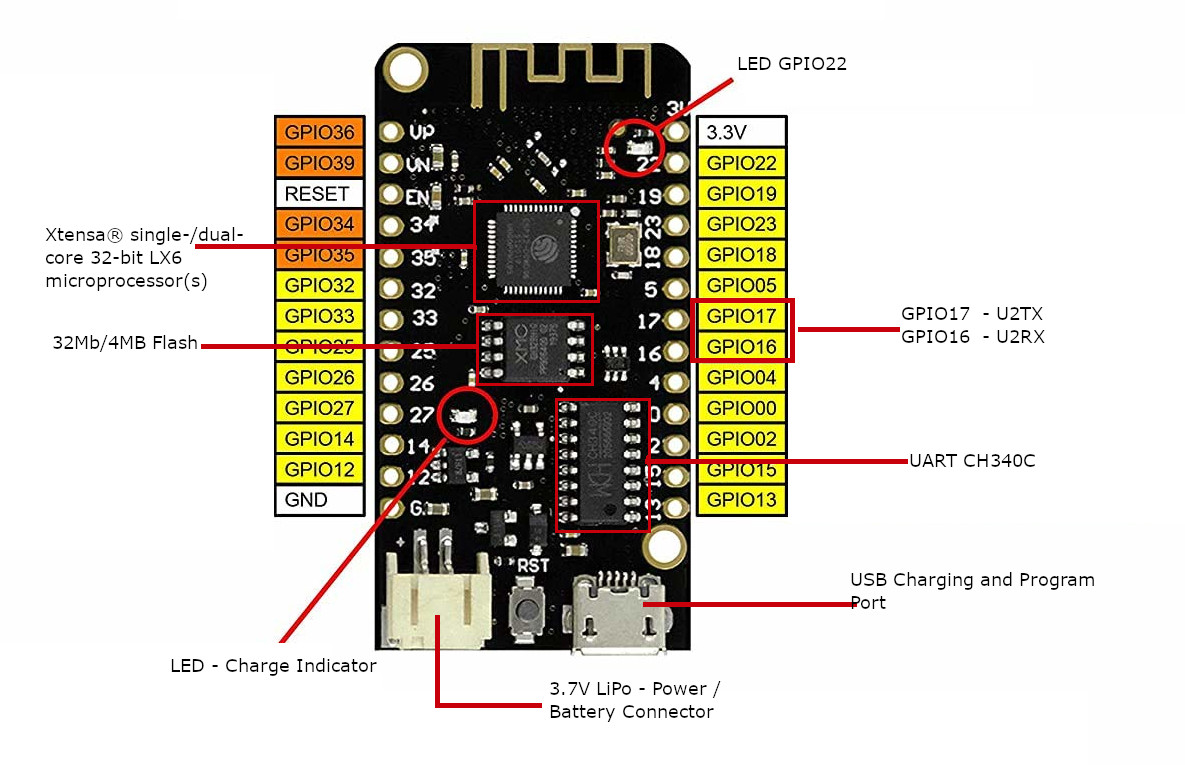
\includegraphics[width=0.99\textwidth]{images/fp/esp32final_edited.jpg}
    \caption{ESP32 Low-power Board From Espressif System}
    \label{fig:esp32}
}
\end{figure}

% \begin{table}[H]
%     % \tiny
%     \centering
%     \caption{\label{tbl:esp-spec} Technical Specification of Wemos Lolin32 Lite}
%     % \resizebox{\linewidth}{!}{
%     \begin{NiceTabular}{|p{2.5cm}|p{3cm}|}
%     \CodeBefore
%     % \rowcolors[gray]{2}{0.8}{}[cols=1-2,restart]
%     \Body
%     \toprule
%         Operating voltage &  3.3V \\
%         \hline
%         Supported Battery &	Lipo 3.7V\\
%         \hline
%         Battery Connector & PH-2 2.0mm\\
%         \hline
%         Digital I/O Pins & 22 \\
%         \hline
%          RAM Memory &  512KB\\
%         \hline
%         Clock Speed(Max) &	240MHz \\
%         \hline
%         SPI Flash &	4M Bytes \\
%         \hline
%         Size & 57*25.4mm \\
%     \bottomrule
%     \end{NiceTabular}
%     % }
% \end{table}

One of the key advantages of the Wemos LoLin32 Lite board is that it is supported by both the Arduino and ESP-IDF (Espressif IoT Development Framework) development environments. For our research project, we opted to use the Arduino embedded development framework to implement the ASCON and AES-GCM algorithms using the C and C++ programming languages. In addition, we utilized PlatformIO, an open-source platform for embedded development, to facilitate the building and deployment of our program onto the Wemos LoLin32 Lite board via the serial port.